%%%% Better Poster latex template example v1.0 (2019/04/04)
%%%% GNU General Public License v3.0
%%%% Rafael Bailo
%%%% https://github.com/rafaelbailo/betterposter-latex-template
%%%%
%%%% Original design from Mike Morrison
%%%% https://twitter.com/mikemorrison

\documentclass[a0paper,fleqn]{betterposter}
\usepackage{float}
\usepackage[latin1]{inputenc}
\usepackage{tikz}
\usepackage{booktabs}
\usetikzlibrary{shapes,arrows}
\usetikzlibrary{arrows.meta}

% Define block styles
\tikzstyle{decision} = [diamond, draw, fill=blue!20,
text width=4.5em, text badly centered, node distance=25em, inner sep=0pt]
\tikzstyle{block} = [rectangle, draw, fill=blue!20,
text width=6em, text centered, rounded corners, minimum height=4em, node distance = 15em]
\tikzstyle{line} = [draw, -latex', line width=.5mm]
\tikzstyle{line2} = [draw, -latex', line width=.7mm]
\tikzstyle{cloud} = [draw, ellipse,fill=red!20, node distance=20em,
minimum height=2em]
\tikzstyle{block2} = [rectangle, draw, fill=white!20,
text width=6em, text centered, rounded corners, minimum height=4em, node distance = 10em, text=black]
%%%% Uncomment the following commands to customise the format

%% Setting the width of columns
% Left column
%\setlength{\leftbarwidth}{0.25\paperwidth}
% Right column
%\setlength{\rightbarwidth}{0.25\paperwidth}

%% Setting the column margins
% Horizontal margin
%\setlength{\columnmarginvertical}{0.05\paperheight}
% Vertical margin
%\setlength{\columnmarginhorizontal}{0.05\paperheight}
% Horizontal margin for the main column
%\setlength{\maincolumnmarginvertical}{0.15\paperheight}
% Vertical margin for the main column
%\setlength{\maincolumnmarginhorizontal}{0.15\paperheight}

%% Changing font sizes
% Text font
%\renewcommand{\fontsizestandard}{\fontsize{28}{35} \selectfont}
% Main column font
%\renewcommand{\fontsizemain}{\fontsize{28}{35} \selectfont}
% Title font
%\renewcommand{\fontsizetitle}{\fontsize{28}{35} \selectfont}
% Author font
%\renewcommand{\fontsizeauthor}{\fontsize{28}{35} \selectfont}
% Section font
%\renewcommand{\fontsizesection}{\fontsize{28}{35} \selectfont}

%% Changing font sizes for a specific text segment
% Place the text inside brackets:
% {\fontsize{28}{35} \selectfont Your text goes here}

%% Changing colours
% Background of side columns
%\renewcommand{\columnbackgroundcolor}{black}
% Font of side columns
%\renewcommand{\columnfontcolor}{gray}
% Background of main column
%\renewcommand{\maincolumnbackgroundcolor}{empirical}
%\renewcommand{\maincolumnbackgroundcolor}{theory}
%\renewcommand{\maincolumnbackgroundcolor}{methods}
%\renewcommand{\maincolumnbackgroundcolor}{intervention}
% Font of main column
%\renewcommand{\maincolumnfontcolor}{gray}

\begin{document}

\betterposter{

  %%%%%%%% MAIN COLUMN

  \maincolumn{

    %% Main space

    \textbf{Function-Fiasco} is an automated tool that detects pseudo-tested
    methods in real Python programs.
    %
    \vfill

    \vspace*{-.5in}
    %
    \tikzstyle{thickWhite} = [thick, white, line width=10pt, -{Latex[length=.5in]}]

\begin{tikzpicture}[auto, scale=.5, every node/.style={scale=.4}]

  \node [block2] (Ti) {Test Case \\ \vspace*{-1in} $T_{i}$};
  \node [block2, right of=sys] (file) {Method \\ \vspace*{-1in} $m$};

  \node [block2, right of=file] (Func) {Function- \\ \vspace*{-1in} Fiasco};
  \node [block2, right of=Func] (Pass) {Status of \\ \vspace*{-1in} $T_i$};

  \draw[thickWhite] (Ti) to (file);

  % \path [line2] (Ti) -- (file);
  \path [line2] (file) -- (Func);
  \path [line2] (Func) -- (Pass);

\end{tikzpicture}

    %
    \vspace*{-2.5in}

    Does the status of $T_i$ change when Function-Fiasco does not run $m$?
    %
    \vspace*{-4.5in}

    }{

    %%%% Bottom space

    %% QR code
    %
    \qrcode{img/qr_code}{img/smartphoneWhite}{
      \textbf{Scan the QR Code} to
      \\visit our GitHub project

    }

  }

  }{
  %%%%%%%% LEFT COLUMN

  \title{\fontsize{50}{60}\selectfont Automatic Detection of Pseudo-tested Methods using Python and Pytest}
  \author{Nicholas Tocci}
  \author{Gregory Kapfhammer}

  \section{Introduction}
  Software systems are very large and complex. Due to this, modern Python
  programs are difficult to test due to the lack of type safety. This could cause a psuedo-tested methods to exist in Python programs. A
  psuedo-tested method is method that is tested, but which passes regardless of the
  output of a function. Function-Fiasco helps determine how much of
  the code is adequately tested and provides a metric that is more representative of
  the actual conditions of the system.
  \section{Implementation}
  % Linear regression
  % Author: Henri Menke
  % Retrieved from: http://www.texample.net/tikz/examples/linear-regression/

  \centering\nointerlineskip
  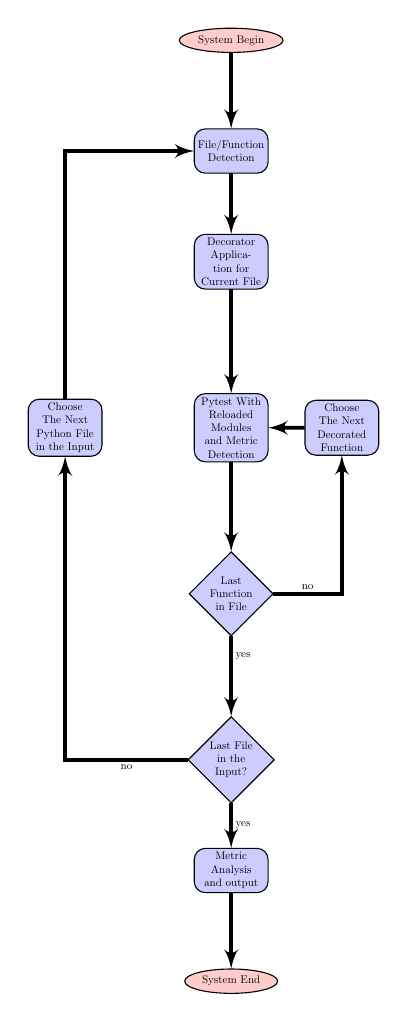
\begin{tikzpicture}[auto, scale=5, every node/.style={scale=0.4}]
    \node [cloud] (sys) {System Begin};
    \node [block, below of=sys, node distance=10em] (file) {File/Function Detection};
    \node [block, below of=file, node distance=10em] (Decorator) {Decorator Application for Current File};
    \node [block, below of=Decorator] (pytest) {Pytest With Reloaded Modules and Metric Detection};
    \node [block, right of=pytest, node distance=10em] (choose) {Choose The Next Decorated Function};
    \node [block, left of=pytest] (Next) {Choose The Next Python File in the Input};
    \node [decision, below of=pytest, node distance=15em] (function) {Last Function in File};
    \node [decision, below of=function, node distance=15em] (Last) {Last File in the Input?};
    \node [block, below of=Last, node distance=10em] (Metric) {Metric Analysis and output};
    \node [cloud, below of=Metric, node distance=10em] (end) {System End};


    \path [line] (sys) -- (file);
    \path [line] (file) -- (Decorator);
    \path [line] (Decorator) -- (pytest);
    \path [line] (pytest) -- (function);
    \path [line] (choose) -- (pytest);
    \path [line] (function) -| node [near start] {no} (choose);
    \path [line] (function) -- node [near start] {yes} (Last);
    \path [line] (Last) -| node [near start] {no} (Next);
    \path [line] (Next) |- (file);
    \path [line] (Last) -- node {yes} (Metric);
    \path [line] (Metric) -- (end);

\end{tikzpicture}


  %% Institution logo

  }{

  %%%%%%%% RIGHT COLUMN

  \section{Preliminary Results}

  \begin{table}[H]
\centering

\huge

% \begingroup\small

% \begin{tabular}{rlrrrrrrrrr}
%   \hline

%  & Program & Coverage & Function Cov & NUMM & NUMTM & Fiascoed & Pseudo & NUMTTM & UC & Change \\
%   \hline

%   1 & Hashids-Python & 0.97 & 0.94 &  16 &  15 &  10 &  8 &   7 & 0.44 & 0.50 \\

%   2 & Bleach & 0.48 & 0.41 & 368 & 152 &   8 &   2 & 150 & 0.41 & 0.00 \\

%   3 & Pycco & 0.77 & 0.86 &  22 &  19 &   6 &   5 &  14 & 0.64 & 0.22 \\

%   4 & Howdoi & 0.78 & 0.95 &  20 &  19 &   2 &   0 &  19 & 0.95 & 0.00 \\

%   5 & Flashtext & 0.81 & 0.33 &  42 &  14 &   7 &   4 &  10 & 0.24 & 0.09 \\

%   6 & Honcho & 0.85 & 0.69 &  58 &  40 &   7 &   5 &  35 & 0.60 & 0.09 \\

%   7 & Maya & 0.90 & 0.50 &  88 &  44 &  13 &   3 &  41 & 0.47 & 0.03 \\

%   8 & Gator & 0.99 & 0.86 &  92 &  79 &  54 &  30 &  49 & 0.53 & 0.33 \\

%   9 & Hatch & 1.00 & 0.56 & 134 &  75 &  14 &   6 &  69 & 0.51 & 0.05 \\

%   10 & Nikola & 0.67 & 0.44 & 732 & 319 &  16 &   9 & 310 & 0.42 & 0.02 \\

%    \hline

% \end{tabular}

\begin{tabular}{r|cccc}
  % \hline

  % OLD:
  %  & Program & Coverage & Function Cov & NUMM & NUMTM & Fiascoed & Pseudo & NUMTTM & UC & Change \\
  %  \hline

  Program & Coverage & Total & Modified & Pseudo-Tested \\
  \hline

  % OLD:
  % 1 & Hashids-Python & 0.97 & 0.94 &  16 &  15 &  10 &  8 &   7 & 0.44 & 0.50 \\
  %
  Hashids-Python & 97\% & 16 & 10 & 8 \\

  % 2 & Bleach & 0.48 & 0.41 & 368 & 152 &   8 &   2 & 150 & 0.41 & 0.00 \\

  % 3 & Pycco & 0.77 & 0.86 &  22 &  19 &   6 &   5 &  14 & 0.64 & 0.22 \\

  % 4 & Howdoi & 0.78 & 0.95 &  20 &  19 &   2 &   0 &  19 & 0.95 & 0.00 \\

  % 5 & Flashtext & 0.81 & 0.33 &  42 &  14 &   7 &   4 &  10 & 0.24 & 0.09 \\

  % 6 & Honcho & 0.85 & 0.69 &  58 &  40 &   7 &   5 &  35 & 0.60 & 0.09 \\

  % 7 & Maya & 0.90 & 0.50 &  88 &  44 &  13 &   3 &  41 & 0.47 & 0.03 \\

  % 8 & Gator & 0.99 & 0.86 &  92 &  79 &  54 &  30 &  49 & 0.53 & 0.33 \\

  % 9 & Hatch & 1.00 & 0.56 & 134 &  75 &  14 &   6 &  69 & 0.51 & 0.05 \\

  % 10 & Nikola & 0.67 & 0.44 & 732 & 319 &  16 &   9 & 310 & 0.42 & 0.02 \\

   % \hline

\end{tabular}


% \endgroup



\end{table}


  Function-Fiasco detects pseudo-tested methods in real Python programs.

  \section{Future Work}
  %
  Add new features to Function-Fiasco: \\
  %
  \vspace*{-.5in}

  \begin{itemize}[leftmargin=*]

    \item{Improve type fuzzing capability}
      %
    \item{Better observe parameterized tests}
      %
    \item{Calculate more types of test coverage}

  \end{itemize}

  \vspace{.5em}
  %
  Use Function-Fiasco to study and improve pseudo-tested methods.

  \section{Conclusion}
  %
  Pseudo-tested methods exist in many real-world Python programs.
  %
  Function-Fiasco automatically detects these methods, saving time that testers
  can instead devote to improving test suites.
  %
  Available on GitHub, Function-Fiasco aids the implementation of high-quality
  Pytest test suites and Python programs.

  \section{Get Involved}
  %
  If you would like support the development of Function-Fiasco, please raise an
  issue on the tracker on or create a pull request to add a new feature or bug
  fix.
  %
  \vfill

  \section{Acknowledgements}
  %
  Poster creation aided by Cory Wiard.\\

  \vspace*{.5in}

  
\includegraphics[width=\textwidth]{img/ComputerScience-Stack}

}

\end{document}
